\section{Elektrische Komponenten}

\begin{frame}
	
	%todo weglassen und auf DMC-folie erwähnen?
	%todo falls verwendet, text mit bilder ersetzen!
	
	\frametitle{Servos und Smart Servos}
	%Als Aktoren wurden verschiedene gewöhnliche Servos und Smart Servos verwendet:
	%\begin{itemize}
	%	\item Modellbauservo: Mini Maestro Servo Controller
	%	\item Smart Servo: \textit{Dynamixel AX-12A}, Halfduplex-UART, Serieschaltung
	%\end{itemize}
	
	\vspace{-2em}
	
	\begin{columns}[t]
		\column{0.5\textwidth}
		\begin{figure}
			\centering
			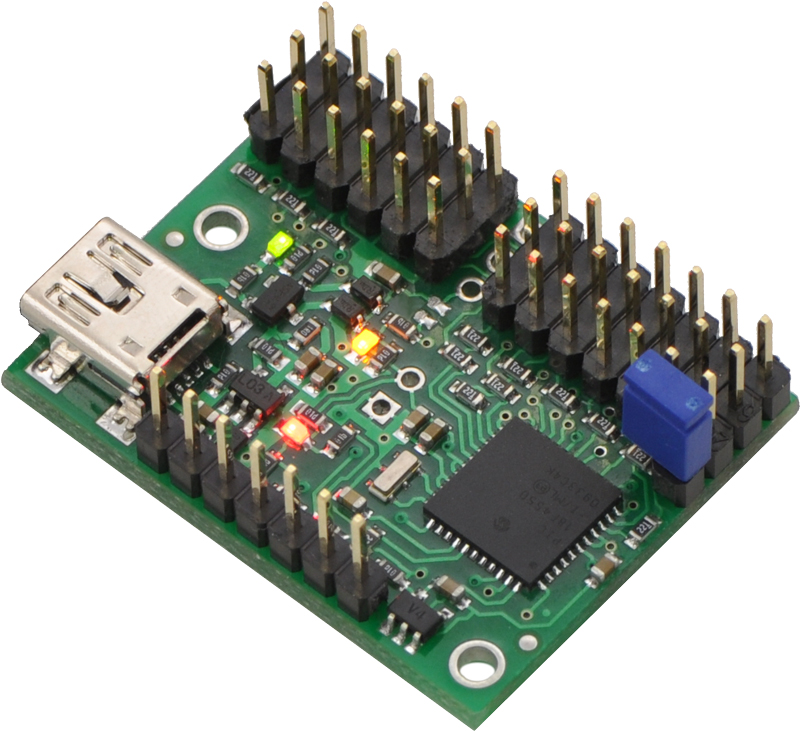
\includegraphics[width=0.7\columnwidth]{../images/maestroServoController.jpg}
			\caption{Quelle: www.pololu.com/product/1352}
		\end{figure}
		\column{0.5\textwidth}
		\begin{figure}
			\centering
			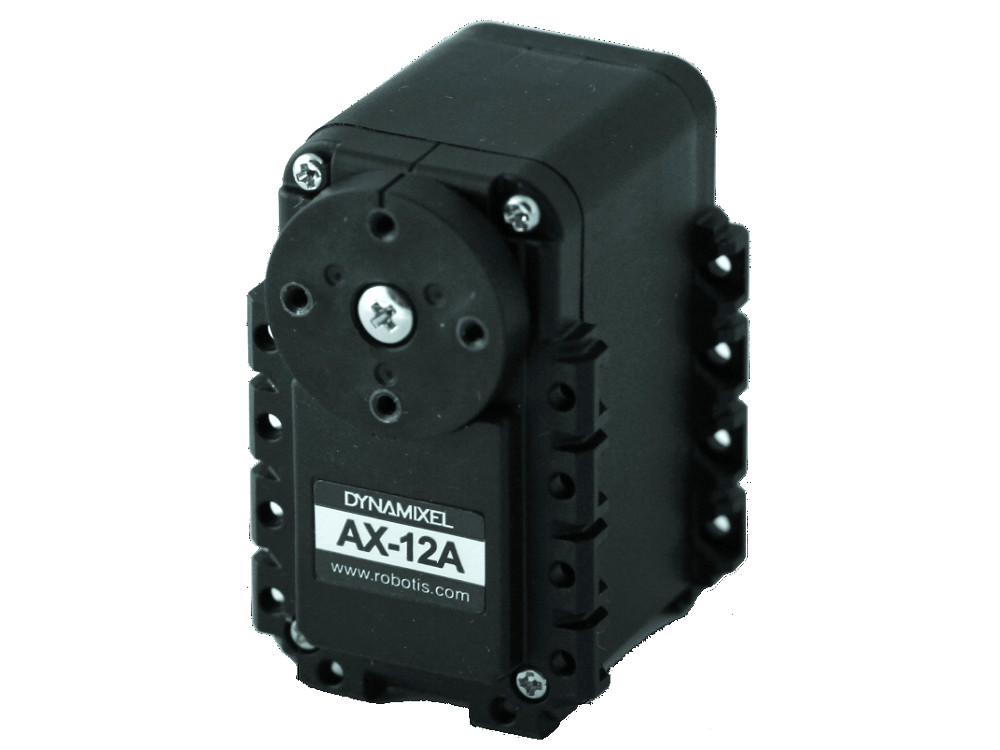
\includegraphics[width=0.9\columnwidth]{../images/dynamixelAX12A.jpg}
			\caption{Quelle: www.eu.diigiit.com/dynamixel-ax-12a}
		\end{figure}
	\end{columns}
	
\end{frame}

\begin{frame}
	\frametitle{Dual Motor Controller}
	
	\begin{columns}[T]
		\begin{column}{0.45\textwidth}
			\begin{center}
				\begin{itemize}
					\item Regelung von 2 DC Motoren
					\item Kommunikation via CAN Bus
					\item Problem: schwache Treiberstufe
				\end{itemize}
			\end{center}
		\end{column}
		\begin{column}{0.45\textwidth}
			\begin{figure}
				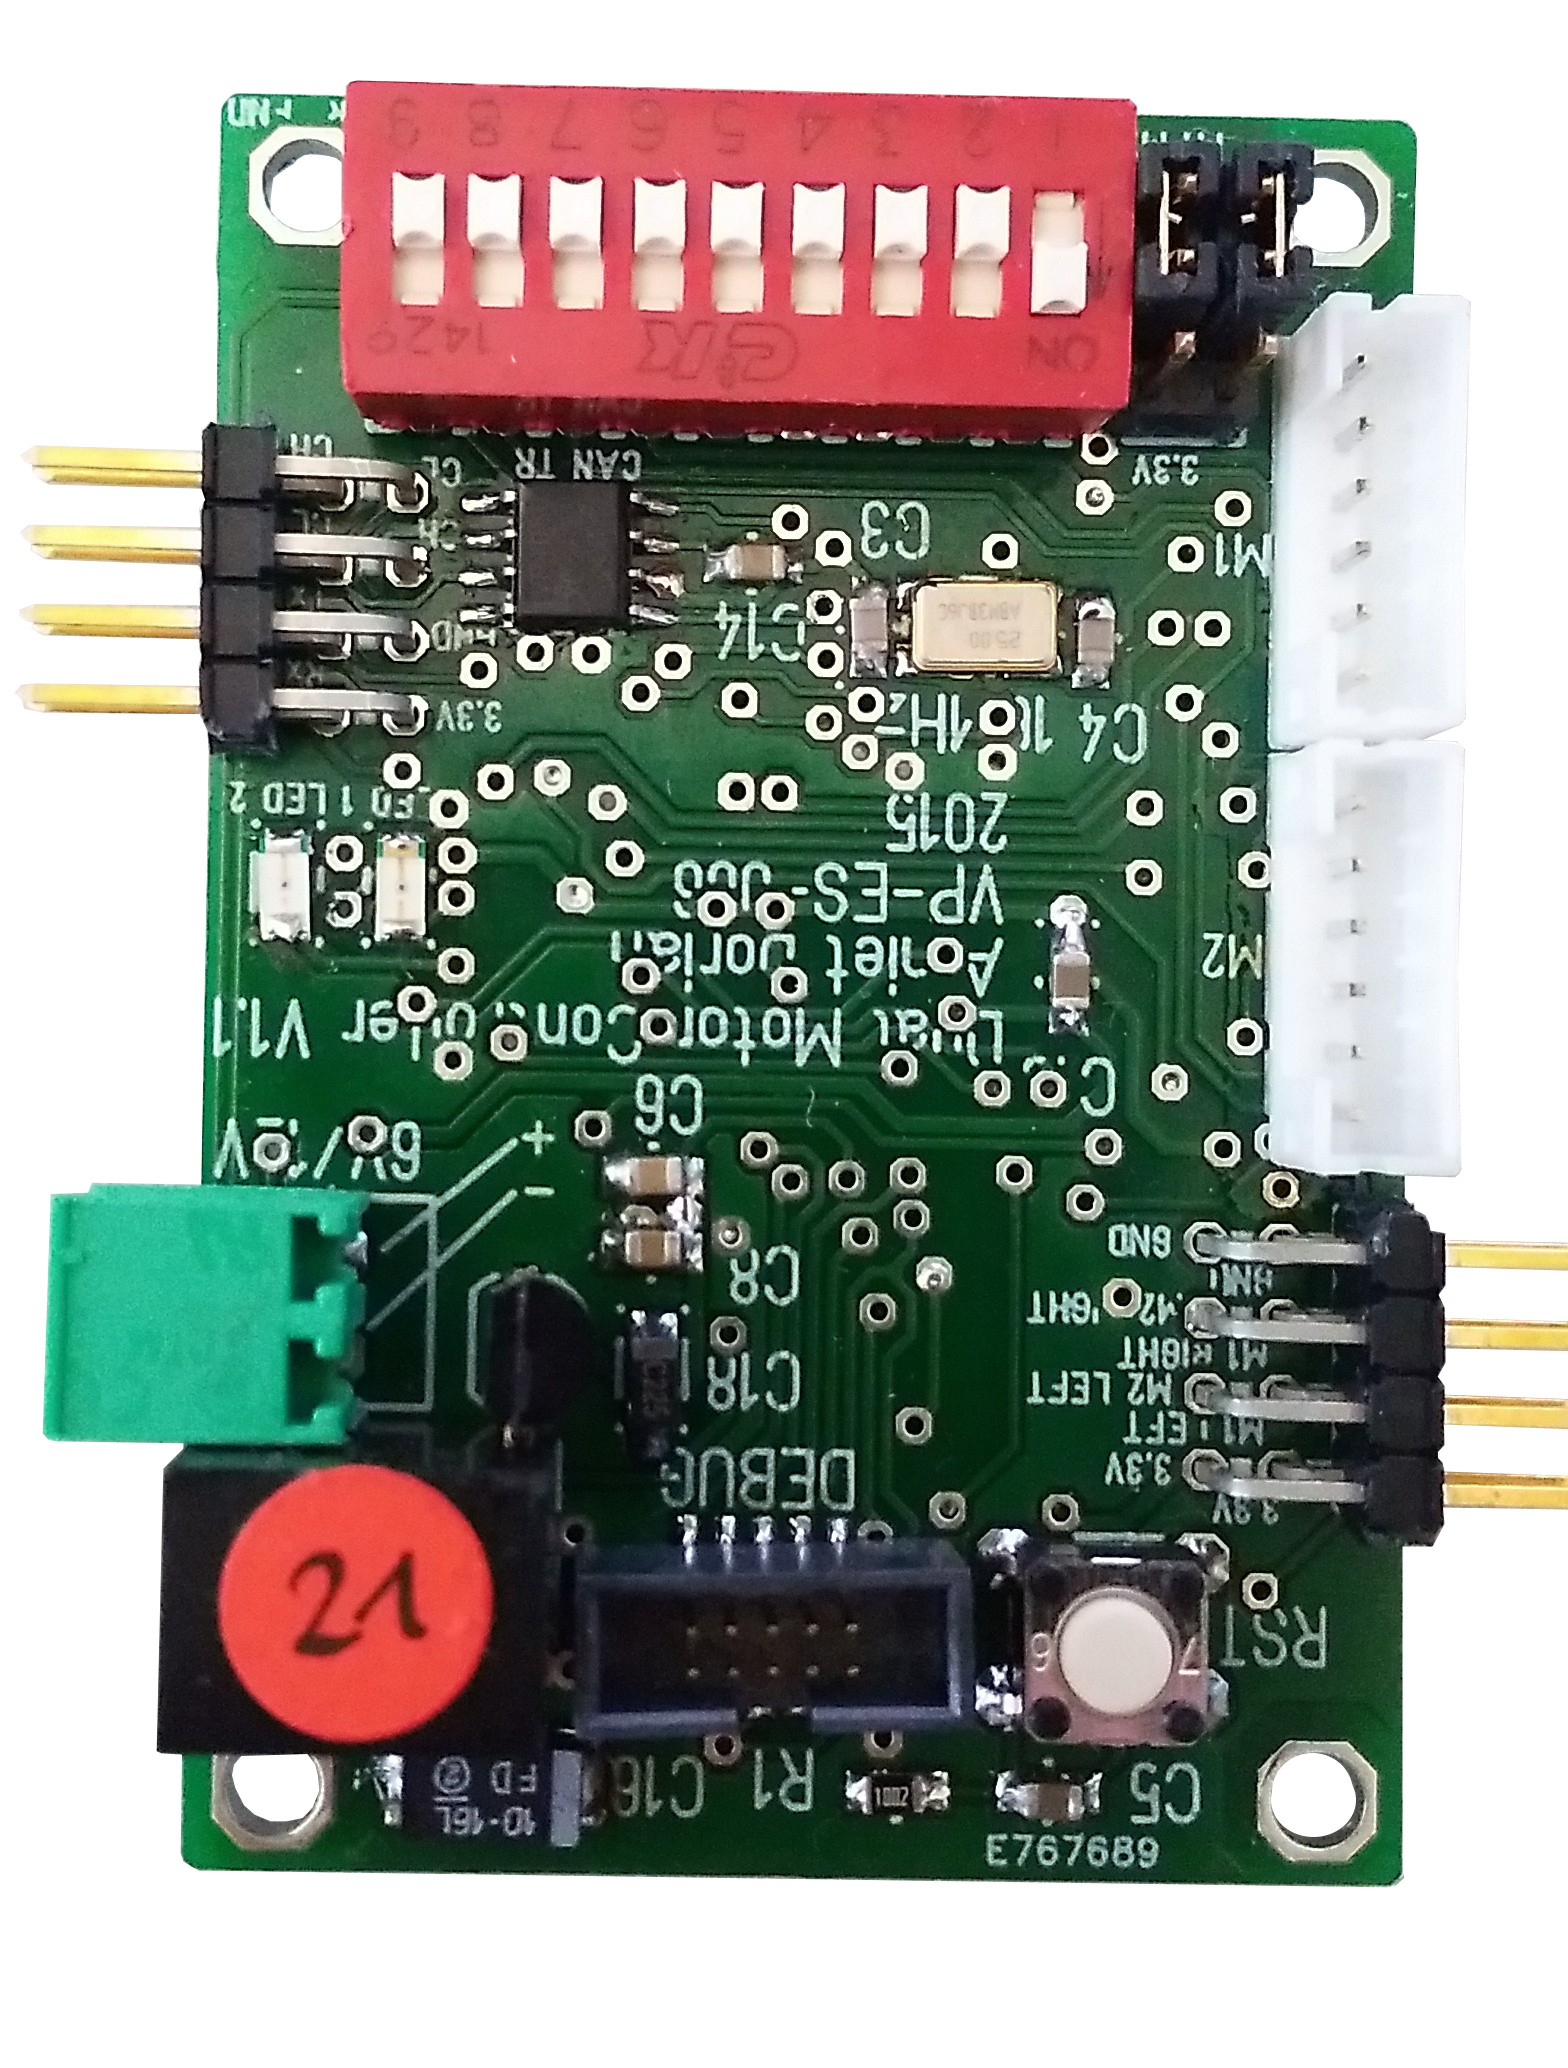
\includegraphics[width=0.7\columnwidth, angle=180, origin=c]{../images/presentation/DMC.jpg}
			\end{figure}
		\end{column}
	\end{columns}
	
\end{frame}

\begin{frame}
	\frametitle{Farbsensor}
	
	\begin{itemize}
		\item Erste Auswahl des Sensors: \textit{Adafruit TCS34725}
		\item Probleme mit I\textsuperscript{2}C
		\item Zweite Auswahl: \textit{Optek OPB780Z}
		\item Frequenzmoduliertes Signal
	\end{itemize}
	
\end{frame}
